% !Mode:: "TeX:UTF-8"
%!TEX program  = xelatex

\documentclass{cumcmthesis}
%\documentclass[withoutpreface,bwprint]{cumcmthesis} %去掉封面与编号页

\usepackage{url}
\usepackage[style=caspervector,backend=biber,utf8]{biblatex}
\addbibresource{文献数据库.bib}
\title{全国大学生数学建模竞赛编写的LaTeX模板}
\tihao{A}	%选题
\baominghao{4321}	%队伍编号
\schoolname{武汉理工大学}	%学校
\membera{刘子川}	%队员1
\memberb{XXX}	%队员2
\memberc{XXX}	%队员3
\supervisor{老师}	%指导老师
\yearinput{2019}	%日期
\monthinput{07}
\dayinput{09}

\begin{document}
	
	\maketitle
	
	\begin{abstract}
		第一段:针对自己选择的题目,说明自己用了什么方法来解决的(这类题属于哪种典型的问题),其中利用了哪些关键的算法,再说出自己的所建模型的创新点。没有创新点,也可以说自己所建的模型相比较于其它的是一个很好的方案。
		
		第二段:问题一中,针对具体问题,进行分析和求解,几句话介绍自己是怎么解决的,有数字结果的也可以直接贴结果。
		
		第三段:问题二中,类比于第二段。
		
		第四段:问题三中,类比于第三段。
		
		第五段:问题四中,类比于第四段。
		
		第六段:如果有问题五,类比于第五段,没有就结束,也可以写一下团队的想法。
		
		\textbf{摘要只能写一面 务必占满这一面!!}
		
		\keywords{折叠桌\quad  曲线拟合\quad   非线性优化模型\quad  受力分析}
	\end{abstract}
	
	%目录
	\tableofcontents
	\newpage	%换页符
	
	\section{问题重述}
	\subsection{问题的背景}
	创意平板折叠桌注重于表达木制品的优雅和设计师所想要强调的自动化与功能性。为了增大有效使用面积。设计师以长方形木板的宽为直径截取了一个圆形作为桌面,又将木板剩余的面积切割成了若干个长短不一的木条,每根木条的长度为平板宽到圆上一点的距离,分别用两根钢筋贯穿两侧的木条,使用者只需提起木板的两侧,便可以在重力的作用下达到自动升起的效果,相互对称的木条宛如下垂的桌布,精密的制作工艺配以质朴的木材,让这件工艺品看起来就像是工业革命时期的机器。
	
	\subsection{问题的提出}
	
	围绕创意平板折叠桌的动态变化过程、设计加工参数,本文依次提出如下问题:
	
	(1)给定长方形平板尺寸 ($120 cm \times 50 cm \times 3 cm$),每根木条宽度(2.5 cm),连接桌腿木条的钢筋的位置,折叠后桌子的高度(53 cm)。要求建立模型描述此折叠桌的动态变化过程,并在此基础上给出此折叠桌的设计加工参数和桌脚边缘线的数学描述。
	
	(2)......


	\section{模型的假设}
	\begin{itemize}
		\item 忽略实际加工误差对设计的影响;
		\item 木条与圆桌面之间的交接处缝隙较小,可忽略;
		\item 钢筋强度足够大,不弯曲;
		\item 假设地面平整。
	\end{itemize}


	\section{符号说明}
	\begin{center}
		\begin{tabular}{cc}
			\hline
			\makebox[0.3\textwidth][c]{符号}	&  \makebox[0.4\textwidth][c]{意义} \\ \hline
			D	    & 木条宽度(cm) \\ \hline
			L	    & 木板长度(cm)  \\ \hline
			W	    & 木板宽度(cm)  \\ \hline
			N	    & 第n根木条  \\ \hline
			T	    & 木条根数  \\ \hline
		\end{tabular}
	\end{center}


	\section{模型准备(可选)}
	背景知识背景知识背景知识背景知识背景知识背景知识背景知识背景知识背景知识背景知识背景知识背景知识背景知识背景知识背景知识背景知识背景知识背景知识背景知识背景知识背景知识


	
	\section{问题的分析}
	\subsection{问题一 xxx}
	\subsubsection{问题描述和分析}
	题目要求建立模型描述折叠桌的动态变化图,由于在折叠时用力大小的不同,我们不能描述在某一时刻折叠桌的具体形态,但我们可以用每根木条的角度变化来描述折叠桌的动态变化。首先,我们知道折叠桌前后左右对称,我们可以运用几何知识求出四分之一木条的角度变化。最后,根据初始时刻和最终形态两种状态求出桌腿木条开槽的长度。
	
	问题流程图:
	\begin{figure}[!h]
		\centering
		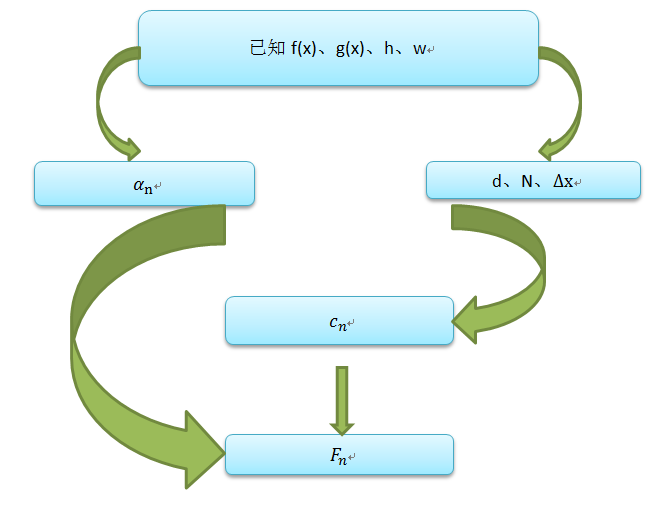
\includegraphics[width=.6\textwidth]{1.png}
		\caption{问题三流程图}
	\end{figure}
	
	\subsubsection{模型建立与求解}
	模型建立与求解模型建立与求解模型建立与求解模型建立与求解模型建立与求解模型建立与求解模型建立与求解模型建立与求解模型建立与求解模型建立与求解模型建立与求解。
	
	表格应具有三线表格式,因此常用 booktabs宏包,其标准格式如表~\ref{tab001}~所示。
	\begin{table}[!htbp]
		\caption{标准三线表格}\label{tab001} \centering
		\begin{tabular}{ccccc}
			\toprule[1.5pt]
			$D$(in) & $P_u$(lbs) & $u_u$(in) & $\beta$ & $G_f$(psi.in)\\
			\midrule[1pt]
			5 & 269.8 & 0.000674 & 1.79 & 0.04089\\
			10 & 421.0 & 0.001035 & 3.59 & 0.04089\\
			20 & 640.2 & 0.001565 & 7.18 & 0.04089\\
			\bottomrule[1.5pt]
		\end{tabular}
	\end{table}


	这里是引用文献的方法:\parencite{王瑶2017基于}

	
	这里是引用文献的方法:\parencite{王瑶2017基于}

			
	这里是引用文献的方法:\parencite{王瑶2017基于}

	
	\textbf{图片格式}
	\begin{figure}[h]
		\centering
		
\includegraphics[width=5cm]{gongzhonghao.jpg}
		\caption{图片标题}
	\end{figure}


	\textbf{矩阵}


	$$
	\begin{matrix}
		1 & x & x^2 \\
		1 & y & y^2 \\
		1 & z & z^2 \\
	\end{matrix} \qquad
	\begin{pmatrix}
		1 & x & x^2 \\
		1 & y & y^2 \\
		1 & z & z^2 \\
	\end{pmatrix}
	$$
	
	\textbf{多行数学公式}
	
	\begin{gather}
%	gather(代编号) 和gather*(不代编号) 环境(可使用\\换行)
		a + b = b + a \\
		ab ba
	\end{gather}
	\begin{gather}
		\imath \vdots \left ( \left \langle ssa \right \rangle \right )
	\end{gather}
	
%	$$
%	\begin{align}
%	\frac{\partial J(\theta)}{\partial\theta_j}
%	& = -\frac1m\sum_{i=0}^m(y^i-h_\theta(x^i)) \frac{\partial}{\partial\theta_j}(y^i-h_\theta(x^i)) \\
%	& = -\frac1m\sum_{i=0}^m(y^i-h_\theta(x^i)) \frac{\partial}{\partial\theta_j}(\sum_{j=0}^n\theta_jx_j^i-y^i) \\
%	& = -\frac1m\sum_{i=0}^m(y^i-h_\theta(x^i))x^i_j
%	\end{align}
%	$$
%	
	
	\subsection{问题二 xxx}
	\subsubsection{问题描述和分析}
	问题的分析问题的分析问题的分析问题的分析问题的分析问题的分析问题的分析问题的分析问题的分析问题的分析问题的分析问题的分析问题的分析问题的分析。
	\subsubsection{模型建立与求解}
	模型建立与求解模型建立与求解模型建立与求解模型建立与求解模型建立与求解模型建立与求解模型建立与求解模型建立与求解模型建立与求解模型建立与求解模型建立与求解。
	
	\subsection{问题三 xxx}
	\subsubsection{问题描述和分析}
	问题的分析问题的分析问题的分析问题的分析问题的分析问题的分析问题的分析问题的分析问题的分析问题的分析问题的分析问题的分析问题的分析问题的分析。
	\subsubsection{模型建立与求解}
	模型建立与求解模型建立与求解模型建立与求解模型建立与求解模型建立与求解模型建立与求解模型建立与求解模型建立与求解模型建立与求解模型建立与求解模型建立与求解。
	
	\subsection{问题四 写作参考格式}

	写写作过程中可能要用到一些格式参考,正式写作的时候,可以直接将这一章删掉即可。写作过程中可能要用到一些格式参考,正式写作的时候,可以直接将这一章删掉即可。写作过程中可能要用到一些格式参考,正式写作的时候,可以直接将这一章删掉即可。写作过程中可能要用到一些格式参考,正式写作的时候,可以直接将这一章删掉即可。写作过程中可能要用到一些格式参考,正式写作的时候,可以直接将这一章删掉即可。作过程中可能要用到一些格式参考,正式写作的时候,可以直接将这一章删掉即可。

	\bigskip
	table环境是一个将表格嵌入文本的浮动环境。
	tabular环境的必选参数由每列对应一个格式字符所组成:c表示居中,l表示左对齐,r表示右对齐,其总
	个数应与表的列数相同。此外,\verb|@{文本}|可以出现在任意两个上述的列格式之间,其中的文本将被插入每一行
	的同一位置。表格的各行以\verb|\\|分隔,同一行的各列则以\&分隔。
	\verb|\toprule|、\verb|\midrule|和\verb|\bottomrule|三个命令是由booktabs宏包提供的,其
	中\verb|\toprule|和\verb|\bottomrule|分别用来绘制表格的第一条(表格最顶部)和第三条(表格最底部)水平线,
	\verb|\midrule|用来绘制第二条(表头之下)水平线,且第一条和第三条水平线的线宽为1.5pt,第二条水平线的线宽为1pt。
	引用方法:“如表~\verb|\ref{标签名}|~所示”。

	\section{模型的评价}
	\subsection{模型的优点}
	模型的优点模型的优点模型的优点模型的优点模型的优点模型的优点模型的优点模型的优点模型的优点模型的优点模型的优点模型的优点模型的优点模型的优点。
	\subsection{模型的缺点}
	模型的缺点模型的缺点模型的缺点模型的缺点模型的缺点模型的缺点模型的缺点模型的缺点模型的缺点模型的缺点模型的缺点模型的缺点模型的缺点模型的缺点。 
	模型的缺点模型的缺点模型的缺点模型的缺点模型的缺点模型的缺点模型的缺点模型的缺点模型的缺点模型的缺点模型的缺点模型的缺点模型的缺点模型的缺点。 
	模型的缺点模型的缺点模型的缺点模型的缺点模型的缺点模型的缺点模型的缺点模型的缺点模型的缺点模型的缺点模型的缺点模型的缺点模型的缺点模型的缺点。 
	模型的缺点模型的缺点模型的缺点模型的缺点模型的缺点模型的缺点模型的缺点模型的缺点模型的缺点模型的缺点模型的缺点模型的缺点模型的缺点模型的缺点。 
	

\newpage	%换页符
%%参考文献
%\begin{thebibliography}{9}%宽度9
% \setlength{\itemsep}{-2mm}
\nocite{*}		%排版未引用的参考文献
\printbibliography[title = {参考文献}]	%使用国标参考文献添加方式

% \bibitem{bib:one} 
% 韩中庚. 数学建模方法及其应用[M]. 高等教育出版社, 2005.
% \bibitem{bib:two}
% 韩中庚. 数学建模方法及其应用[M]. 高等教育出版社, 2005.
% \bibitem{bib:two}
% 韩中庚. 数学建模方法及其应用[M]. 高等教育出版社, 2005.
% 
% \nocite{*}		%排版未引用的参考文献
% \bibliography{文献数据库}	%不同书库用数据分割
%
%\end{thebibliography}

\newpage
%附录
\begin{appendices}
\section{排队算法--matlab 源程序}
\begin{lstlisting}[language=matlab]
kk=2;[mdd,ndd]=size(dd);
while ~isempty(V)
[tmpd,j]=min(W(i,V));tmpj=V(j);
for k=2:ndd
[tmp1,jj]=min(dd(1,k)+W(dd(2,k),V));
tmp2=V(jj);tt(k-1,:)=[tmp1,tmp2,jj];
end
tmp=[tmpd,tmpj,j;tt];[tmp3,tmp4]=min(tmp(:,1));
if tmp3==tmpd, ss(1:2,kk)=[i;tmp(tmp4,2)];
else,tmp5=find(ss(:,tmp4)~=0);tmp6=length(tmp5);
if dd(2,tmp4)==ss(tmp6,tmp4)
ss(1:tmp6+1,kk)=[ss(tmp5,tmp4);tmp(tmp4,2)];
else, ss(1:3,kk)=[i;dd(2,tmp4);tmp(tmp4,2)];
end;end
dd=[dd,[tmp3;tmp(tmp4,2)]];V(tmp(tmp4,3))=[];
[mdd,ndd]=size(dd);kk=kk+1;
end; S=ss; D=dd(1,:);
 \end{lstlisting}
 \section{规划解决程序--lingo源代码}
\begin{lstlisting}[language=c]
kk=2;
[mdd,ndd]=size(dd);
while ~isempty(V)
    [tmpd,j]=min(W(i,V));tmpj=V(j);
for k=2:ndd
    [tmp1,jj]=min(dd(1,k)+W(dd(2,k),V));
    tmp2=V(jj);tt(k-1,:)=[tmp1,tmp2,jj];
end
    tmp=[tmpd,tmpj,j;tt];[tmp3,tmp4]=min(tmp(:,1));
if tmp3==tmpd, ss(1:2,kk)=[i;tmp(tmp4,2)];
else,tmp5=find(ss(:,tmp4)~=0);tmp6=length(tmp5);
if dd(2,tmp4)==ss(tmp6,tmp4)
    ss(1:tmp6+1,kk)=[ss(tmp5,tmp4);tmp(tmp4,2)];
else, ss(1:3,kk)=[i;dd(2,tmp4);tmp(tmp4,2)];
end;
end
    dd=[dd,[tmp3;tmp(tmp4,2)]];V(tmp(tmp4,3))=[];
    [mdd,ndd]=size(dd);
    kk=kk+1;
end;
S=ss;
D=dd(1,:);
 \end{lstlisting}
\end{appendices}

\end{document} 


%其绘制表格的代码及其说明如下。
%\begin{tcode}
%	\begin{table}[!htbp]
%		\caption[标签名]{中文标题}
%		\begin{tabular}{cc...c}
%			\toprule[1.5pt]
%			表头第1个格   & 表头第2个格   & ... & 表头第n个格  \\
%			\midrule[1pt]
%			表中数据(1,1) & 表中数据(1,2) & ... & 表中数据(1,n)\\
%			表中数据(2,1) & 表中数据(2,2) & ... & 表中数据(2,n)\\
%			...................................................\\
%			表中数据(m,1) & 表中数据(m,2) & ... & 表中数据(m,n)\\
%			\bottomrule[1.5pt]
%		\end{tabular}
%	\end{table}
%\end{tcode}